%=========================================================================%
% - - - KAPITOLA 3: J U N I T                                             %
\chapter{Testovací rámec JUnit}                                           %
%=========================================================================%
JUnit je jednoduchý nástroj pro psaní testů a testování aplikací. Jeho vývoj je založen na otevřeném zdrojovém kódu (\emph{angl. open-source}), a proto lze najít množství dalších nástrojů, které rámec JUnit používají nebo z~něj vycházejí. Cílem JUnit je poskytovat nástroj, který by umožňoval \cite{JUnitGuide}:
\begin{description}
  \item[Jednoduchost psaní testů:]
  programátor nemusí psát zbytečně mnoho kódu, zbytek za něj vykoná rámec JUnit.
  \item[Snadné pochopení rámce JUnit:]
  rámec by měl být pro Javu přirozený, tak aby se programátor naučil s~rámcem pracovat co nejrychleji.
  \item[Rychlé provedení testů:]
  spouštění jednotlivých testovacích případů by mělo probíhat bez zbytečných odkladů tak, aby šetřilo programátorům čas.
  \item[Izolované provedení testů:]
  rámec by měl poskytovat izolaci jednotlivých testovacích případů, která zajišťuje dostatečnou stabilitu testovacích sad.
  \item[Skládat a provádět různé kombinace testů:]
  lze spustit například testy se stejným štítkem\,(\emph{angl. tag}) nebo jen vybrané testy v~sadě.
\end{description}

Bohužel jsou některé z~těchto podmínek v~rozporu mezi sebou a tak nelze splnit všechny tyto požadavky v plném rozsahu. V~této kapitole je popsán testovací rámec JUnit, jeho architektura, aplikační rozhraní, vybraná existující rozšíření a zásuvné moduly postavené na tomto rámci. 


  \section{Architektura rámce JUnit}
  %=================================
  V~roce 1999 publikoval Kent Beck svůj rámec pro jednotkové testování pro programovací jazyk Smalltalk\,--\,\emph{SmalltalkUnit} (zkráceně SUnit). Idea tohoto rámce spočívá v~nalezení ideální kombinace mezi jednoduchostí a užitečností. Později Erich Gamma přepsal SUnit do jazyka Java a vytvořil tak JUnit. Posléze tak začaly vznikat mnohé obdoby rámce JUnit podporující mnohé programovací jazyky \cite{UnitTestFrameworks}:

  \begin{description}
   \item[CppUnit:] pro jazyk C++
   \item[CUnit:] pro jazyk C
   \item[NUnit:] pro jazyk .NET, včetně C\#, VB.NET, J\# a Managed C++
   \item[PyUnit:] pro jayzk Python
   \item[vbUnit:] pro jazyk Visula Basic
   \item[utPLSQL:] pro jazyk PL/SQL od firmy Oracle
   \item[MinUnit:] minimalistická verze pro jazyk C
  \end{description}


    \subsection{xUnit}
    %*****************
    Všechny rámce založené na xUnit se drží stejných základů. Klíčovými třídami v~každém rámci jsou třídy \emph{TestCase}, \emph{TestRunner}, \emph{TestFixture}, \emph{TestSuite} a \emph{TestResult} \cite{UnitTestFrameworks}.

    \begin{description}
      \item[TestCase] je základní třídou reprezentující jednotkový test. Všechny jednotkové testy jsou odvozeny od této třídy a dědí její vlastnosti.
      \item[TestRunner] je třída spouštějící jednotlivé testy a zpracovávající jednotlivé výsledky. Existují dva základní typy runnerů -- grafický a textový. Nejdůležitější metodou je metoda \texttt{run()}, která spouští runner a testy zadané jako parametr této metody.
      \item[TestFixture] je třída umožňující izolaci jednotlivých testovacích případů. Redukuje množství napsaného kódu a izoluje jednotlivé testovací případy tak, aby průběh jednoho nebyl závislý na výsledku druhého. V zásadě jde o poskytnutí metod, které připraví prostředí před během testovací sady nebo testovacího případu, poté zase vrátí prostředí do původního stavu a uvolní alokované zdroje.
      \item[TestSuite] je třída sloužící k seskupení množství jednotlivých testovacích případů i sad -- umožňuje tak spouštět vybrané testovací případy a sady najednou.
      \item[TestResult] je třída sloužící pro získání výsledků o běhu testů. Instance této třídy se předává jako parametr metody \texttt{run()} (u tříd TestCase i TestSuite). Tato třída uchovává data jako jsou počet běhů testovacích případů, informace o chybách (běhových i testových) a informace o jednotlivých testovacích případech.
    \end{description}


    \subsection{JUnit}
    \label{section:JUnit}
    %*****************
    Architektura testovacího rámce (viz obrázek \ref{fig:junit_arch}) JUnit se od xUnit liší jen v maličkostech. Obsahuje pět základních tříd, které vytváří aplikační rozhraní rámce: Assert, Test, TestCase, TestSuite, TestResult.

    Třída Assert poskytuje kolekci metod sloužících pro ověření výsledků testovacích případů. Tyto metody jsou statické a většinou se volají přímo z daného testovacího případu. Slouží pro porovnání hodnot proměnných a umožňují zadat vlastní zprávu, která je v případě chybné hodnoty vypsána na standardní chybový výstup. V takovém případě je testovací případ ukončen a kód za metodou není vykonán.

    Třída Test je rozhraní implementované všemi třídami, které se chovají jako testy. Definuje dvě základní metody\,--\,\texttt{countTestCases()} a \texttt{run()}. První zmíněná metoda vrací počet testovacích případů v dané třídě, druhá spustí testy a jejich výsledky ukládá do instance třídy TestResult, předaného jako parametr metody \texttt{run()}. Obyčejně toto rozhraní implementují třídy TestCase a TestSuite.

    Třída TestCase představuje jeden testovací případ. Metoda \texttt{countTestCases()} tedy vrací číslo 1 a metoda \texttt{run()} spustí tři fáze: \uv{set-up}, testovací metoda a \uv{tear-down}. Díky těmto částem lze dosáhnout lepší izolovatelnosti provedení jednotlivých testovacích případů. Výsledek je zaznamenán do instance typu TestResult (parametrem metody \texttt{run()}).

    Třída TestSuite je kolekcí dalších testů implementujících rozhraní Test. Může tak obsahovat jak jednoduché testovací případy typu TestCase, tak celé testovací sady TestSuite (popřípadě i jiné objekty implementující rozhraní Test). Většina IDE implicitně vytváří testovací sady a tak není potřeba je explicitně definovat.

    Jak již bylo dříve zmíněno, třída TestResult slouží k uchování výsledků testů. Jedná se o data jako počet běhů testovacích případů, počet běhových chyb, počet testových chyb, detailnější informace o jednotlivých chybách a podobně. Na konci běhu testů tak instance třídy TestResult obsahuje kompletní seznam informací o proběhlých testech. JUnit také poskytuje užitečný nástroj, jakým lze instanci typu TestResult sledovat - \emph{listener}. Jedná se o způsob sledování obsahu instance TestResult a v případě změny je pak daný listener o této události uvědoměn. Přidáním vlastního listeneru pomocí metody \texttt{addListener()} uvědomíme JUnit o skutečnosti, že má tomuto listeneru posílat data spojená s určitou instancí třídy TestResult \cite{JUnitGuide}.

    \begin{figure}
      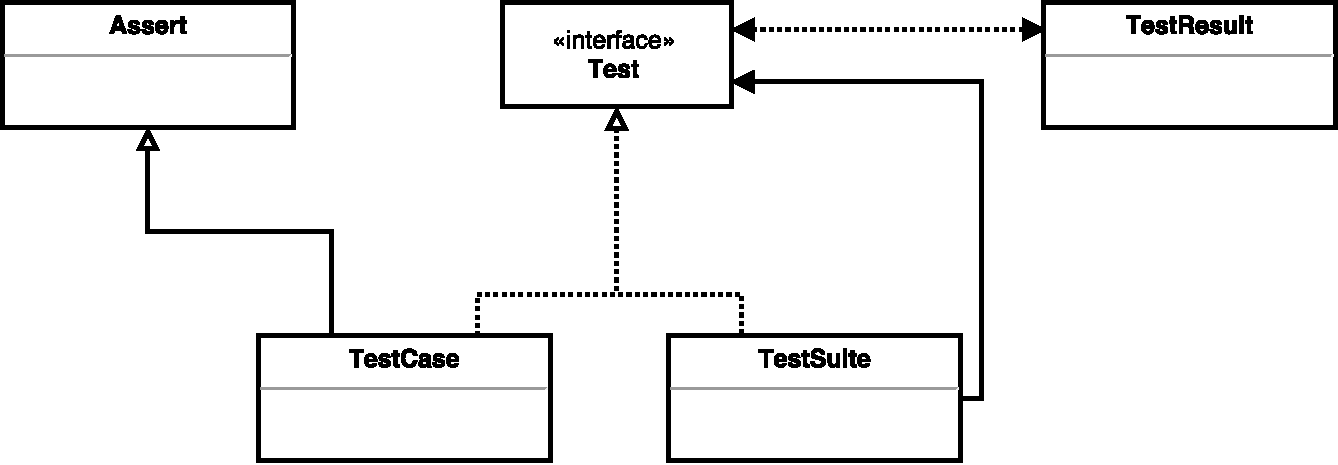
\includegraphics[width=\textwidth, center]{obrazky-figures/junit_arch.pdf}
      \caption{Struktura testovacího rámce JUnit. (převzato z knihy \cite{JUnitGuide}, strana 21)}
      \label{fig:junit_arch}
    \end{figure}


  \section{Aplikační rozhraní rámce JUnit}
  %=======================================
  V následující části se nachází stručný popis aplikačního rozhraní testovacího rámce JUnit včetně vytváření vlastních testovacích sad, použití parametrizovaných tříd a definice pravidel.

    \subsection{Testovací třídy v~rámci JUnit}
    Testovací třída v~rámci Junit je třída obsahující jednotlivé testovací případy. Konvencí pro pojmenování jednotlivých tříd je použití sufixu \uv{Test}. Jednotlivé testovací případy jsou od ostatních metod odlišeny anotací \texttt{@Test}. Díky tomu rámec JUnit pozná jednotlivé testy, které má spustit. Jména metod jednotlivých testovacích případů by měla reflektovat jejich účel.  \cite{vogella:JUnit}. Seznam anotací, které lze v testovací třídě použít je uveden v tabulce \ref{tab:junit_annotations}. \todo{Tabulka}

    \begin{table}
      \centering
      \begin{tabular}{|l|l|}
	\hline
	\textbf{@Test} & Označí metodu jako testovací případ.\\ \hline
	\textbf{@Before} & \begin{tabular}{@{}l@{}}Metoda s touto anotací je zavolána před\\ každým testovacím případem.\\Obyčejně se používa pro připravu prostředí před během každého testovacího případu.\end{tabular}\\ \hline
	\textbf{@After} & vyznam\\ \hline
	\textbf{@BeforeClass} & vyznam\\ \hline
	\textbf{@AfterClass} & vyznam\\ \hline
	\textbf{@Ignore} & vyznam\\ \hline
	\textbf{@Ignore ("Důvod")} & vyznam\\ \hline
	\textbf{@Test (expected = Exception.class)} & vyznam\\ \hline
	\textbf{@Test (timeout = 100)} & vyznam\\
	\hline
      \end{tabular}
      \label{tab:junit_annotations}
      \caption{Seznam anotací použitelných v testovací třídě JUnit. (převzato z \cite{vogella:JUnit})}
    \end{table}


    \subsection{Testovací sady v~rámci JUnit}
    Většina vývojových prostředí umí vytvářet testovací sady automaticky při spouštění (například z vytvořeného projektu). Vývojové prostředí najde všechny testy nacházející se hierarchicky pod spuštěných uzlem a vytvoří z nich testovací sadu. To ovšem nemusí vždy vyhovovat našemu použití a tak lze vytvářet vlastní testovací sady a seskupovat různé testovací třídy dle naší potřeby. Testovací sada se definuje pomocí anotace \texttt{@SuiteClasses}. Jako parametr anotace je zadán seznam jednotlivých testovacích tříd, které do testovací sady patří. Spuštěním testovací sady se spustí všechny testovací třídy a v nich uvedené testovací případy \cite{vogella:JUnit}. Do vytvořené testovací sady lze přidávat nejen třídy s testovacími případy, ale také třídy obsahující testovací sady. Před třídu lze navíc doplnit anotaci \texttt{@RunWith} specifikující runner, který bude při běhu testů použit. Pokud tato informace není uvedena, je použit výchozí runner.

    \subsection{Parametrizované testovací třídy}
    JUnit umožňuje vytvoření parametrizované třídy s vícehodnotovými parametry. Tato třída musí obsahovat pouze jednu metodu s anotací \texttt{@Test} a statickou metodu s anotací \texttt{@Parameters}. Statická metoda je využita k předávání různých hodnot parametrů. Parametry jsou globální proměnné označené anotací \texttt{@Parameter}. Testovací případ je poté spuštěn pro každou uvedenou hodnotu parametru \cite{vogella:JUnit}.

    \subsection{Definice pravidel pro testovací případy}
    Pomocí anotace \texttt{@Rule} je možné upravit chování jednotlivých testovacích příkazů. Pomocí těchto pravidel\footnote{Seznam těchto pravidel lze najít na \url{https://github.com/junit-team/junit4/wiki/Rules}.} lze například vytvářet dočasné složky, externí zdroje nebo třeba definovat očekávanou chybu. JUnit také umožňuje definici vlastních pravidel \cite{vogella:JUnit}.

  \section{Rozšíření rámce JUnit}
  %==============================
  Pro pohodlnější testování a jednodušší psaní testovacích případů je vhodné si JUnit upravit. Použité třídy rámce JUnit jsou poměrně jednoduché a není problém je rozšířit. Pro většinu případů postačí vytvoření nové třídy rozšiřující třídu \texttt{TestCase}. Tím se docílí úpravy jednotlivých testovacích případů a může se tak vytvořit množství specializovaných tříd. Pokud tato změna není dostatečná, lze implementovat rozhraní \texttt{Test}, které poskytuje větší flexibilitu. Pomocí třídy \texttt{TextDecorator} lze obalit testovací případ nebo sadu do bloku a vykonat před nebo po tomto bloku vlastní kód. Dále lze vytvořit vlastní třídy se statickými metodami použitelnými pro vlastní ověření hodnot proměnných, podobně jako ve třídě \texttt{Assert} \cite{JUnitGuide}.

  Markantnějších změn je možno dosáhnout pomocí tříd \texttt{TestResult} a \texttt{TestListener}. Pomocí rozšíření třídy \texttt{TestResult} je možné předat upravenou třídu jako parametr metody \texttt{run()}. Tento přístup umožňuje získaní dalších specifických informací o běhu testů. Nejjednodušším způsobem jak získat informace o běžících testech je ovšem vytvořit vlastní třídu implementující rozhraní \texttt{TestListener} a připojit ji k dané instanci třídy \texttt{TestResult} \cite{JUnitGuide}. Tento způsob je použit při implementaci výsledné aplikace a detailní použití je popsáno v kapitole \ref{chapter:TRV}.

  Další možnou úpravou je vytvoření vlastního runneru. Tato změna poskytuje rozsáhlou kontrolu nad běžícími testy a jejich vykonávání \cite{JUnitGuide}. Pro spuštění vlastního runneru je však třeba tuto skutečnost ve zdrojových souborech testů explicitně definovat pomocí dříve zmíněné anotace \texttt{@RunWith}.

  Samozřejmě již existují mnohá rozšíření a tak není vždy potřeba psát si vlastní. Tyto rozšíření se většinou zabývají specifickými aspekty dle účelu a architektury testované aplikace. Mezi nejznámější patří \emph{JUnitPerf}, \emph{HtttpUnit}, \emph{JWebUnit}, \emph{Cactus}, \emph{JFCUnit}, \emph{JXUnit} a \emph{Jester} \cite{JUnitGuide}.

  \section{Zásuvný modul Eclipse IDE rozšiřující rámec JUnit}
  %===========================================================
  Eclipse IDE využívá rámec JUnit pomocí přidání JAR archivu mezi závislosti projektu a zároveň poskytuje vlastní zásuvný modul \texttt{org.eclipse.jdt.junit}, který usnadňuje uživateli práci s rámcem JUnit v prostředí Eclipse IDE. Tento zásuvný modul je součástí JDT (viz sekce \ref{section:Infrastruktura_Eclipse_IDE}) a nabízí například průvodce pro tvorbu nových testovacích případů a sad, vlastní systémy pro spouštění testů nebo pohled JUnit.

  Z hlediska implementace výsledné aplikace je důležitá část zásuvného modulu \texttt{org.eclipse.jdt.core}, která poskytuje aplikační rozhraní pro interakci Eclipse IDE s rámcem JUnit. Mimo jiné obsahuje třídu \texttt{TestRunListener} pro implementaci listeneru a několik rozhraní použitých pro předávání informací o průběhu testů. Jedná se především o rozhraní \texttt{ITestCaseElement}, \texttt{ITestElement}, \texttt{ITestRunSession}. Tato rozhraní jsou abstrakcí nad třídami rámce JUnit a v podstatě odpovídají dříve zmíněným třídám \texttt{Test}, \texttt{TestCase} a \texttt{TestSuite} (viz sekce \ref{section:JUnit}).
